\chapter{Vehicle Semantics Extraction}

\label{section:semanticsextraction}


\section{Introduction}

In this chapter, the implementation of the vehicle semantic extraction module is discussed in detail.
First, an atom-based quantization process of the video data is introduced in Section \ref{section:atoms}. This quantization technique was implemented for both phases of \versionOneExt and \versionTwoExt frameworks. Next, the process of obtaining the vehicle's bounding box is discussed briefly in Section \ref{subsection:fundamental}.
The following sections thoroughly describes both of the vehicle semantic extraction modulesin Section \ref{section:semantic_lsh} and Section \ref{section:semantic_chamfer}.

%may be good to add a short paragraph to briefly describe and reinforce what "vehicle semantics extraction" is in relation to the big problem and that two extractions methods are introduced in this research and why two .... along with giving a brief distinction between the two.

As the focus of this work revolves around car park surveillance video footage, colour and motion information are key information used to describe vehicles'activities. With the goal of designing retrieval techniques suitable for car park surveillance footage, an accurate extraction of these information is a crucial component of this work.
While there are several differences between both of the extraction methods introduced in this research, the predominant difference lies with the flexibility of the outputs produced from these extraction modules.
The extracted semantics from the \versionOneExt has similar properties to a \textit{keyword-based} system. Hence, the proposed retrieval technique was placed in a hit-or-miss situation. In order to enhance the retrieval process, the \versionTwoExt utilises probability scores to describe the extracted semantics. Hence, increasing the overall robustness.



\section{Atom-based Quantization}
\label{section:atoms}

As the utilisation of video data is central to this work, there was an urgent need to come up with a way to easily manipulate and represent the video information. As video data can be represented using the 3 dimensional space using \textit{X-axis, Y-axis, \& time-axis}, quantization techniques can be applied to convert the continuous data into discrete data blocks.


\begin{figure}[H]\centering
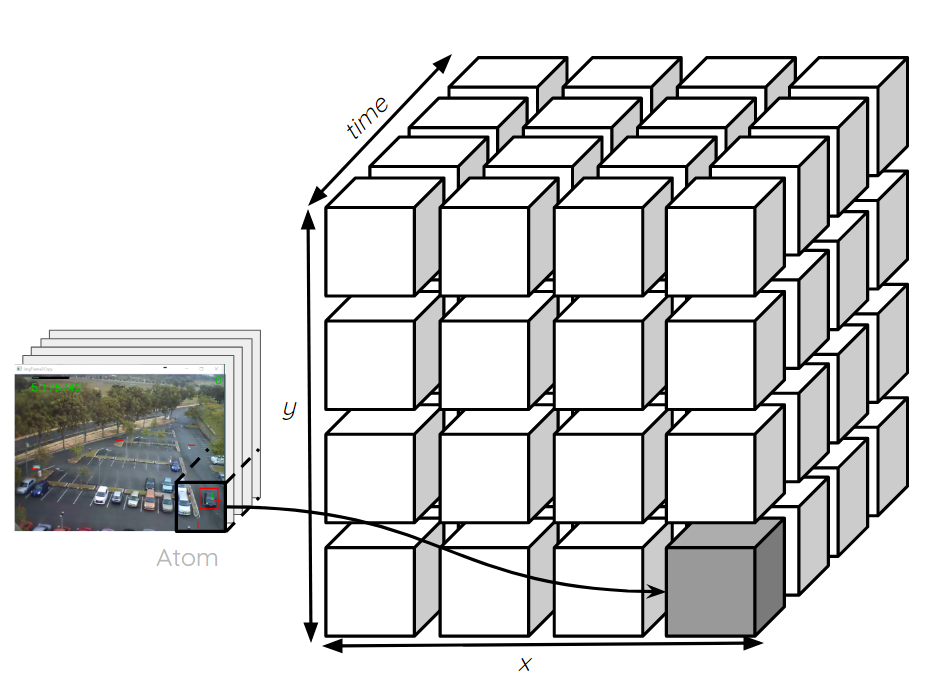
\includegraphics[width=0.6\textwidth]{image/general/atom.PNG}
\caption[Quantization of Video Data into Atoms.]
{Quantization of Video Data into Atoms.
Inspired by the works of \citeA{castanon2016retrieval}.}
\label{fig:atoms}
\end{figure}


In order to design a framework for long-term vehicle semantics extraction from video data, this work adopted the concept of \textbf{"atoms"} as coined by \cite{castanon2016retrieval} which enabled quantization of the video input into individual 3D spatial-temporal cuboids. In this work, an atom is defined as a group of cells at a similar spatial location, that spans a certain fixed number of frames; hence forming a spatio-temporal `cuboid'.
As described in Section \ref{section:dataset_used}, the input video data has a resolution of 640$\times$480 pixels and frame rate of 10$fps$, the dimensions of each atom ($\alpha$) were set to $\alpha_{width}=32$ pixels, $\alpha_{height}=24$ pixels and $\alpha_{time}=10$ frames, which represents the temporal duration of one second. The resolution of the atom ($\alpha_{width},\alpha_{height}$) were set such that the video resolution can be uniformly divided by 20 atoms across both its width and height as illustrated in Figure \ref{fig:viewfromcamera}. Using this setup, each individual atom can be uniquely identified using the $X, Y$ and $T$ identifiers.


However, as mentioned in Section \ref{subsec:vehiclemotionextraction}, the downside of this method is that the accuracy of data representation heavily relies on the number of spatio-temporal cuboids used. With that consideration, the atom's width and height ($\alpha_{width}, \alpha_{height}$) were selected such that one and only one vehicle can occupy a single atom block at any given time. Hence, the colour and trajectory semantics of the vehicles can be adequately represented. While smaller atoms could be used to accurately capture exact location of the vehicle, the additional atoms would only add towards extra computational power needed to process the queries which will be discussed in Chapter \ref{section:retrievalengine}.

The use of these atom-based spatial-temporal cuboids is paramount in this work. By applying the quantization on all axis, the atom-based structure enables two major types of queries to be performed conveniently. Figure \ref{fig:typesofQuery} illustrates the types of queries which are regularly desired when working with video data: \textit{Region of Interest (ROI) query} \& \textit{Time-slicing query}. Typically, the queries used in real world applications are in the form of a combination of both the ROI and time-slicing query where the users are interested in certain activity that occurred in a particular location within a time frame.




\begin{figure}[htb!]
  \centering


\begin{tabular}{cc}
 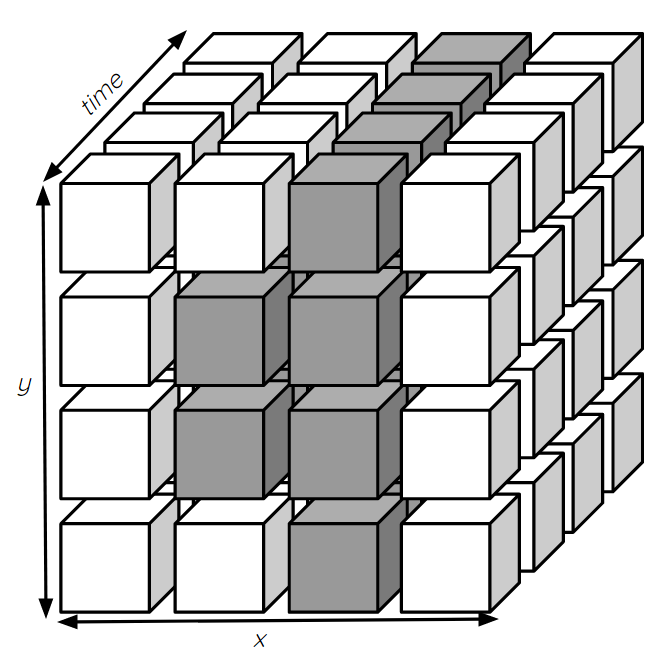
\includegraphics[width=0.3\linewidth]{image/general/atom_ROI.PNG} &  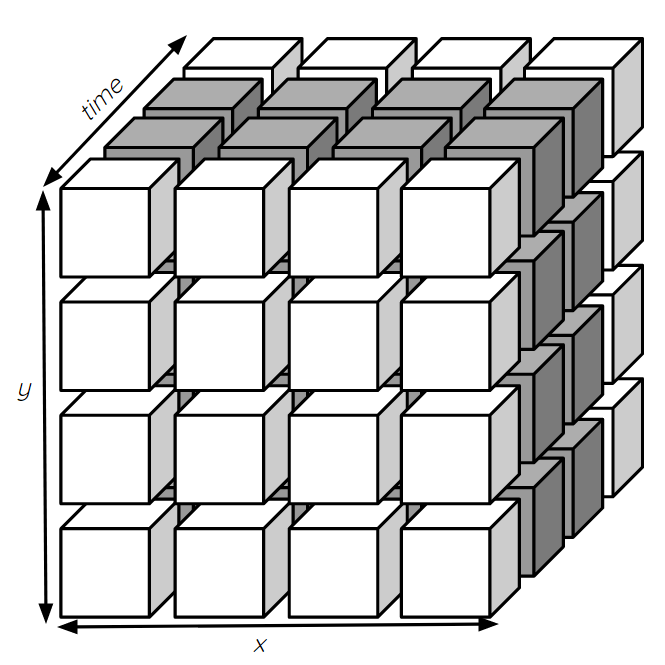
\includegraphics[width=0.3\linewidth]{image/general/atom_time_slicing.PNG}\\
(a) Region of Interest & (b) Time Slicing
\end{tabular}


\caption{Types of Queries} \label{fig:typesofQuery}
\end{figure}



\section{Vehicle Blobs Extraction}
\label{subsection:fundamental}

As described in Section \ref{subsec:scope}, this work assumes that the preliminary task of detecting, tracking and identifying bounding box of each vehicle is obtained prior to the semantic extraction task. This section briefly describes the steps taken by \citeA{lim2017} to detect and extract moving objects in a video using background subtraction techniques to differentiate between static background and moving objects as depicted in Figure \ref{fig:bgs}.

\begin{figure}[htb!]
  \centering
\begin{tabular}{cc}
 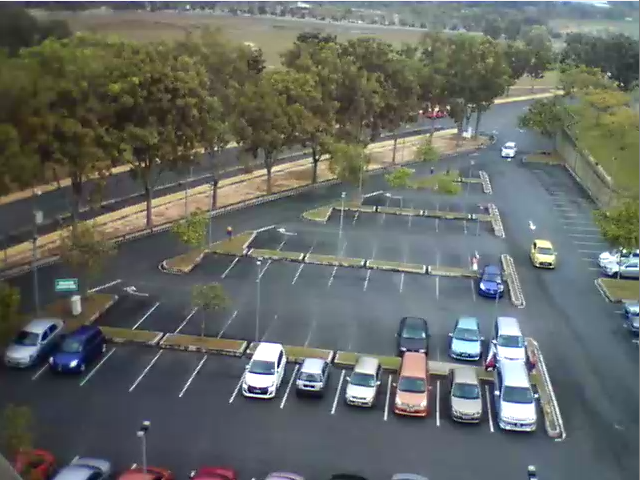
\includegraphics[width=0.4\linewidth]{image/general/bgs1.png} &  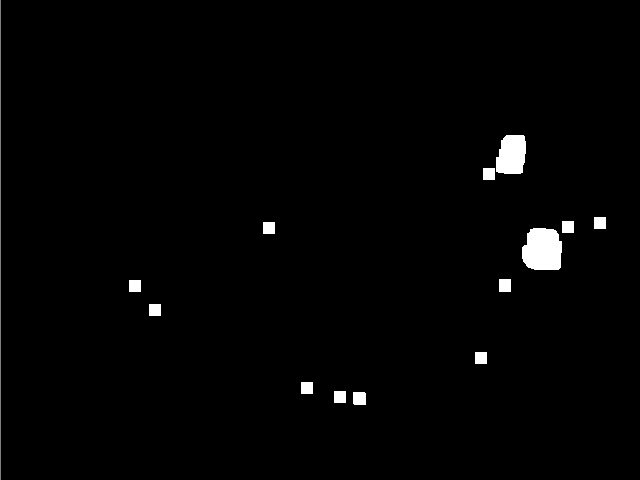
\includegraphics[width=0.4\linewidth]{image/general/bgs2.png}  \\
(a) 123th frame of a video & (b) Result of background subtraction \\
\end{tabular}
\caption{Background Subtraction}
\label{fig:bgs}
\end{figure}

As the vanilla application of background subtraction (BGS) often results with noisy output, the proposed algorithm used in \cite{lim2017} implemented a combination of adaptive learning and frame differencing method. The BGS step was used to detect and extract moving objects (foreground blobs). Several erosion and dilation morphology operations were then performed to further reduce noise and to provide a better representation of foreground blob at the end of the process.
To further improve the accuracy of the extracted blobs, some handcrafted parameters were used to differentiate between vehicles and non-vehicles objects. Furthermore, a deep learning model was deployed to increase the probability of filtering non-vehicle blobs.


\begin{comment}
\begin{figure}[htb!]
  \centering
\begin{tabular}{ccc}
 
\includegraphics[width=0.2\linewidth]{image/general/morph_ori.png} &  
\includegraphics[width=0.2\linewidth]{image/general/morph_erode.png} &
 
\includegraphics[width=0.2\linewidth]{image/general/morph_dilate.png}\\
(a) Original Image & (b) Eroded Image & (c) Dilated Image \\
\end{tabular}
\caption{Morphology Operations: Erosion \& Dilation}
\label{fig:morph}
\end{figure}

The process is known as \textit{Opening} occurs when the morphology operations are done in the following sequence - 1) Erosion, \& 2) Dilation, noisy data from the background subtraction method can be eliminated as the erosion operation will be able to remove noise while maintaining the important subjects. In contrast, the operation known as \textit{closing} occurs when the dilation step is first performed, followed by the erosion step. This process is useful to fill up the gaps within the foreground objects. These processes are illustrated in Figure \ref{fig:morph2}

\begin{figure}[htb!]
  \centering
\begin{tabular}{cc}
 
\includegraphics[width=0.4\linewidth]{image/general/opening.png} &  \includegraphics[width=0.4\linewidth]{image/general/closing.png}  \\
(a) Opening & (b) Closing \\
\end{tabular}
\caption{Morphology Operations: Opening \& Closing}
\label{fig:morph2}
\end{figure}


\cc{do i need to cite these images? \\}
%https://docs.opencv.org/3.0-beta/doc/py_tutorials/py_imgproc/py_morphological_ops/py_morphological_ops.html
\end{comment}


The work of \citeA{redmon2016you} namely YOLOv2 (You Only Look Once) - a deep learning model was deployed as a complementary module. YOLOv2 is a \textbf{real-time} object detection deep learning model, as the detection process incurred very little overhead to the overall computational time and cost.
With the obtained bounding box, each of foreground blobs were used as an input for the YOLOv2 network. The network will then divide the input into multiple smaller regions and perform prediction of the bounding box along with the class probability. As the YOLOv2 model is pre-trained with vehicles as one of the many classes, no further retraining was done. The tracking of the blobs only took place if they were identified as vehicles. These bounding boxes were then fed into the proposed semantic extraction framework for further processing.


\section{Semantic Extraction}
\label{section:semanticsExtraction}

The ability to extract object specific semantics from the scene is able to provide deeper insights for surveillance purposes.

As describe in Section \ref{subsec:scope}, the two major semantics extracted in the proposed algorithm are (i) \textbf{Vehicle Colour} and (ii) \textbf{Vehicle Trajectory}. Other semantic information such as the time and date which were extracted is briefly discussed as these are simple extraction based on the input file names.
Table \ref{table:semantics} provides a list of all the extracted semantics in this work.
In the following subsections, focus is placed on both the colour and motion semantics extraction process and framework.



\begin{table} \centering
\caption {Types of Extracted Semantics and Methods}
\label{table:semantics}
\begin{tabular}{|l|l|l|}
\hline
\textbf{No.} & \textbf{Semantics Type} & \textbf{Method(s)}                                                                                                          \\ \hline
\textbf{1}   & Date                    & Filename data extraction                                                                                                         \\ \hline
\textbf{2}   & Time                    & Filename data extraction                                                                                                         \\ \hline
\textbf{3}   & Colour                   & \begin{tabular}[c]{@{}l@{}}i) Handcrafted Feature \& Distance Estimation (HSV)\\ ii) Distance Estimation (CIELUV)\end{tabular} \\ \hline
\textbf{4}   & Motion                  & \begin{tabular}[c]{@{}l@{}}i) Handcrafted Feature\\ ii) Collection of Centroid \end{tabular}                                \\ \hline
\textbf{5}   & Object Type             & YOLOv2 (described in \ref{objecttype})                                                                                                               \\ \hline
\textbf{6}   & Size                    & Bounding box from Background Subtraction                                                                                                      \\ \hline
\end{tabular}

\end{table}

\subsection{Colour Semantic}
\label{subsec:colorsemantics}

Without a doubt, colour information plays a significant role as a useful semantics as it is often one of the most common information provided by users when tasked to describe objects from a given event in a particular scene.
However, the process of extracting colour information from vehicles accurately is extremely challenging, especially in an outdoor setting. Often, the white balance of the said scene appears differently depending on various factors such as the ambient illumination during the different hours of the day coupled with weather conditions such as cloudy, rainy or sunshine that may affect the overall scene.
Several commercially available product such as 'Nix colour sensor' \cite{nixsensorltd} and 'Adafruit RGB sensor' \cite{adafruit} makes use of an independent calibrated light source as a means to tackle this challenge.

While colour terms are commonly derived from the Munsell Colour system, there are myriads of available colour terms used in different standards as described in Section \ref{section:colourterm}.
This creates a whole lot of problem in the computing field as colour terms are often described with differing definitions and tuple values.
Hence, there is a dire need of determining the best way to extract and represent colour values with its corresponding colour terms.
Inspirations and ideologies were drawn from the Munsell Colour system and applied in this work.
Although the Munsell Colour system provided a significant research contribution for colour terms naming, the irregularity along the chroma and value axis does not translate well in a modern colour space as the modern colour spaces are often uniformly distributed along all axis.

Hence, in order to better represent the colour space, this work used the Hue-Saturation-Value (HSV) colour space for the colour extraction framework.
The use of the HSV colour space is twofold: Firstly, as the HSV colour space closely resembles the Munsell Colour System, it eases the the colour representation.
Secondly the distance between two colours are now intuitive and linear.
In addition, as HSV colour space is commonly used, the conversion between the RGB and HSV colour spaces are seamless and can be easily introduced into the existing framework. Figure \ref{fig:hsvcylinder} provides a visual representation of the HSV colour space.

\begin{figure}[hbt!]\centering
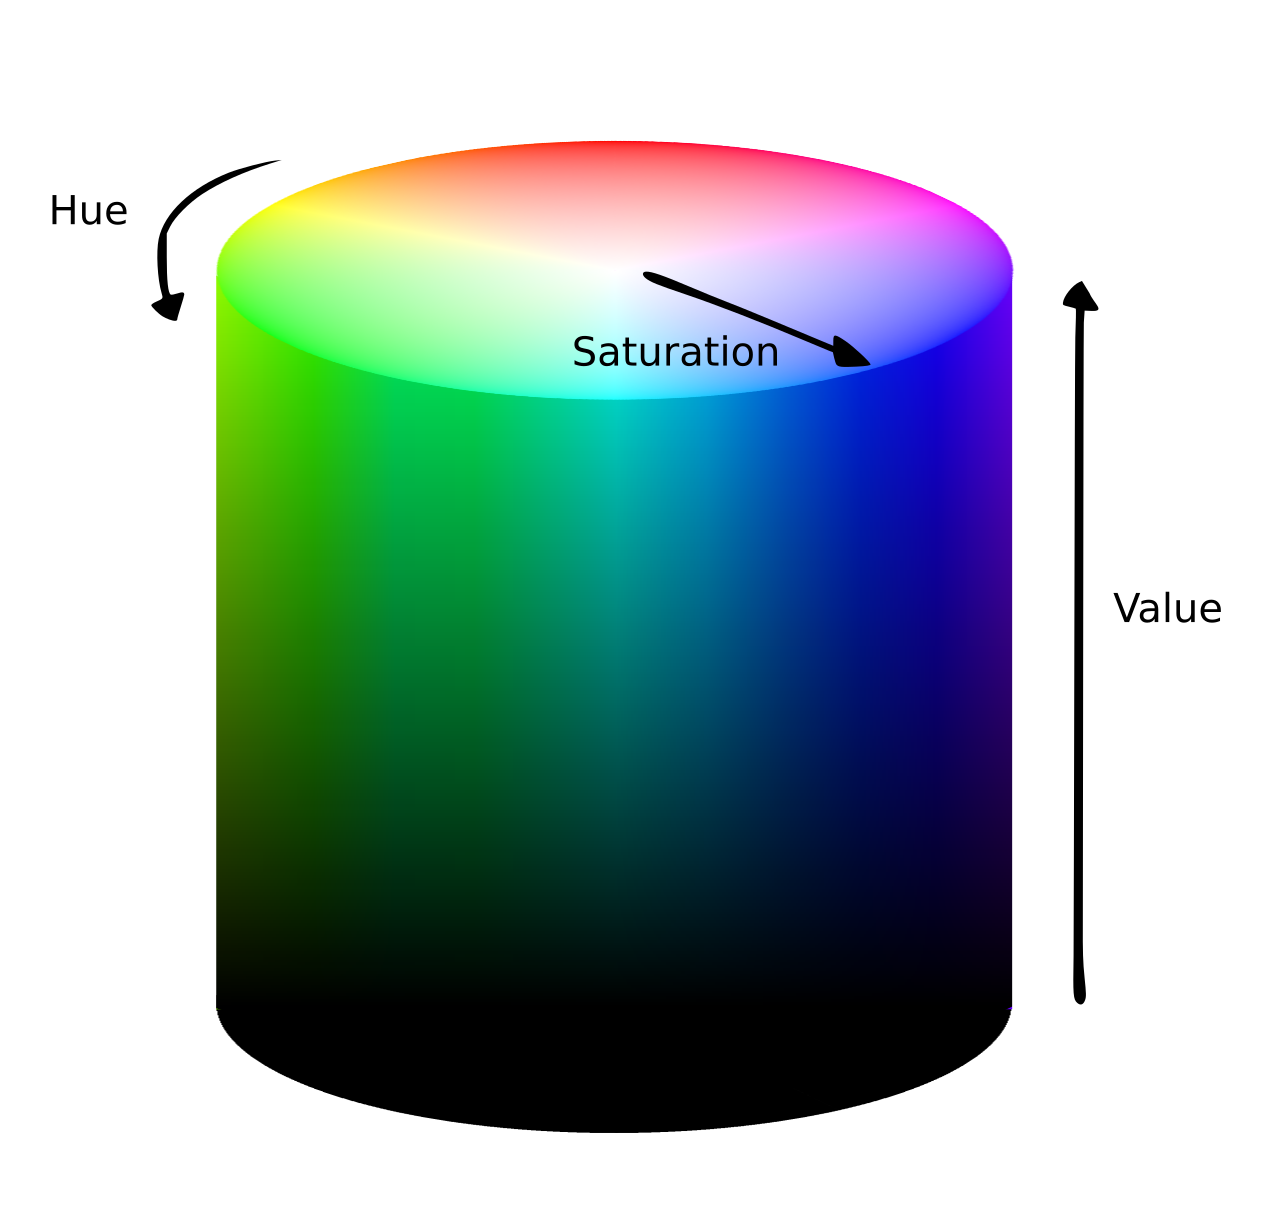
\includegraphics[width=.5\textwidth]{image/general/HSV.png}
\caption{Hue-Saturation-Value (HSV) Cylinder Visualisation}
\label{fig:hsvcylinder}
\end{figure}

Table \ref{table:allcolourterms} lists several famous web colour dictionary along with the number of colour categories available in each of those colour standards. With so many different colour categories, this ultimately leads to the question of "\textit{How many colour categories should be extracted for the colour semantic? And why?}".
Hence, in this work, the eleven basic colour terms in English proposed by \cite{berlinandkay} was adopted.
\citeA{berlinandkay}'s linguistic approach towards the colour terms assures us that these 11 terms sufficiently describes colours which are often used.
However, the definition of colour terms by themselves are insufficient as it invokes another set of challenge - that is, the representation of these colours in \textit{numerical tuples}, such as RGB values which are typically used in computers.
Linking back to the disccusion in Section \ref{section:eyes}, each and every person has a relatively different perception of colour due to the number of cones cells in the retina. This, compounded with the fact that most monitor screens are not colour calibrated professionally provided an opportunity for Munroe \cite{munroe2010color} to perform an internet crowd-sourcing survey on colour terms and their respective numeral representation according to how colours are displayed on typical monitors.

In \citeA{munroe2010color}'s experiments, 222,500 user sessions consisting of 40,000 women and 100,000 men, provided over five million colours according to their respective colour terms. With the collected results, Munroe then proceeds to map RGB tuples to particular colour terms according to the highest response frequency.
According to Munroe, the mapping of these terms were done by averaging results of several stochastic hill climbing algorithms. At the end of the experiment, 954 colour terms were assigned to a set of RGB tuples of equal size. Figure \ref{fig:xkcd} shows the mapping of dominant colour terms over three fully saturated faces of the RGB cube.
Now, by combining the work of Berlin and Kay along with the work of Munroe, the eleven basic colour terms can now be translated into modern colour tuples using the information collected. These colour terms and the corresponding HEX values are listed in Table \ref{table:colorshex} and these values were treated as \textit{ground truth} for each colour term.
The details of the techniques used in the semantics extraction process in Phase 1 and Phase 2 will be discussed further in the subsequent sections.

\begin{figure}[!hbt]\centering
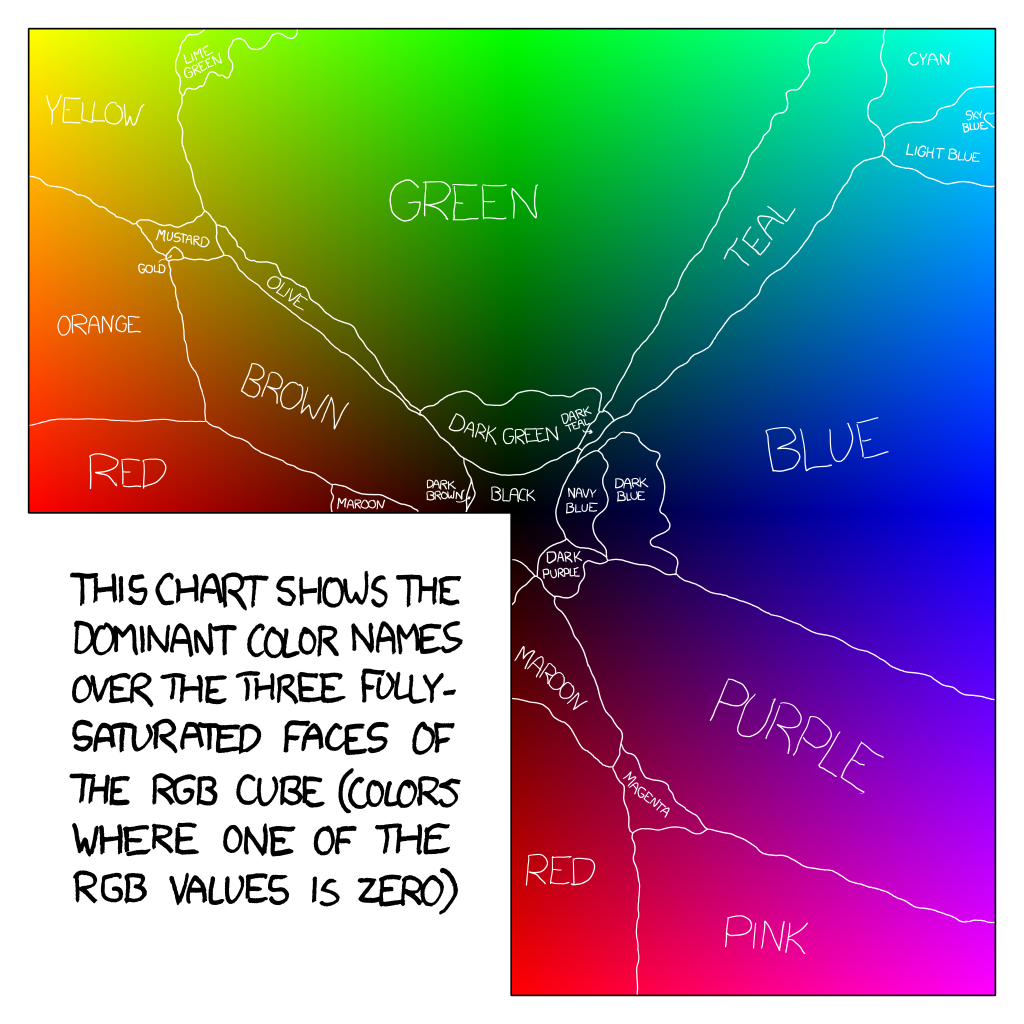
\includegraphics[width=.6\textwidth]{image/general/xkcd.png}
\caption{Dominant Colour Terms over Three Fully Saturated Faces of the RGB Cube}
\label{fig:xkcd}
\end{figure}


% Please add the following required packages to your document preamble:
% \usepackage[table,xcdraw]{xcolor}
% If you use beamer only pass "xcolor=table" option, i.e. \documentclass[xcolor=table]{beamer}
\begin{table}[!ht]\centering
\begin{tabular}{lcccc}
\cline{2-4}
\multicolumn{1}{l|}{}                     & \multicolumn{1}{l|}{\cellcolor[HTML]{000000}} & \multicolumn{1}{l|}{\cellcolor[HTML]{FFFFFF}} & \multicolumn{1}{l|}{\cellcolor[HTML]{929591}} &                                               \\ \cline{1-4}
\multicolumn{1}{|l|}{\textbf{HEX}}        & \multicolumn{1}{c|}{\#000000}                 & \multicolumn{1}{c|}{\#ffffff}                 & \multicolumn{1}{c|}{\#929591}                 &                                               \\ \cline{1-4}
\multicolumn{1}{|l|}{\textbf{Color Term}} & \multicolumn{1}{c|}{Black}                    & \multicolumn{1}{c|}{White}                    & \multicolumn{1}{c|}{Gray}                     &                                               \\ \cline{1-4}
                                          & \multicolumn{1}{l}{}                          & \multicolumn{1}{l}{}                          & \multicolumn{1}{l}{}                          &                                               \\ \cline{2-5}
\multicolumn{1}{l|}{}                     & \multicolumn{1}{l|}{\cellcolor[HTML]{653700}} & \multicolumn{1}{l|}{\cellcolor[HTML]{E50000}} & \multicolumn{1}{l|}{\cellcolor[HTML]{F97306}} & \multicolumn{1}{l|}{\cellcolor[HTML]{FFFF14}} \\ \hline
\multicolumn{1}{|l|}{\textbf{HEX}}        & \multicolumn{1}{c|}{\#653700}                 & \multicolumn{1}{c|}{\#e50000}                 & \multicolumn{1}{c|}{\#f97306}                 & \multicolumn{1}{c|}{\#ffff14}                 \\ \hline
\multicolumn{1}{|l|}{\textbf{Color Term}} & \multicolumn{1}{c|}{Brown}                    & \multicolumn{1}{c|}{Red}                      & \multicolumn{1}{c|}{Orange}                   & \multicolumn{1}{c|}{Yellow}                   \\ \hline
                                          & \multicolumn{1}{l}{}                          & \multicolumn{1}{l}{}                          & \multicolumn{1}{l}{}                          &                                               \\ \cline{2-5}
\multicolumn{1}{l|}{}                     & \multicolumn{1}{l|}{\cellcolor[HTML]{7E1E9C}} & \multicolumn{1}{l|}{\cellcolor[HTML]{15B01A}} & \multicolumn{1}{l|}{\cellcolor[HTML]{0343DF}} & \multicolumn{1}{l|}{\cellcolor[HTML]{FF81C0}} \\ \hline
\multicolumn{1}{|l|}{\textbf{HEX}}        & \multicolumn{1}{c|}{\#7e1e9c}                 & \multicolumn{1}{c|}{\#15b01a}                 & \multicolumn{1}{c|}{\#0343df}                 & \multicolumn{1}{c|}{\#ff81c0}                 \\ \hline
\multicolumn{1}{|l|}{\textbf{Colour Term}}  & \multicolumn{1}{c|}{Purple}                   & \multicolumn{1}{c|}{Green}                    & \multicolumn{1}{c|}{Blue}                     & \multicolumn{1}{c|}{Pink}                     \\ \hline
\end{tabular}
\caption{Colour Terms and the Corresponding HEX value}
\label{table:colorshex}
\end{table}



\subsection{Motion Semantic}

Without a doubt, the use of video data for surveillance purposes lies in its ability to capture motion information. When tasked to describe an action that occured in a given surveillance setting, signs of motion are usually key information provided by users. In this work, the collective motion performed by a vehicle in the scene is defined as a vehicle's trajectory.

Typically, when describing an event, end user uses a combination of several information such as time of occurrence, description of the objects involved, location and the motion occurred. Traditionally, motion information from videos are converted into text based descriptions using handcrafted methods. For instance, an event such as "\textit{A yellow vehicle was turning into the cross section between Road Alpha and Road Beta at 3:30pm when a black vehicle came rushing over and hitting a pedestrian in the process during commotion}" could be converted into a keyword-based statements such as "yellow car turn left Road Alpha and Road Beta".

However, keyword-based statements are not intuitive and easily interpretable for users who are not familiar with the terminology used in the system.
Futhermore, \cite{bhaumik2016hybrid} claims that the use of textual queries has been proven to be ineffective in video retrieval systems because keywords may not be able to capture the type of semantic content required by an end user.
While motions are not as subjective as the concept of colours, text based descriptions of motion events are less intuitive when compared to a graphical description.
Hence, this work aims to extract motion information such that it can be represented using a graphical form, with the goal of providing a naturally more intuitive representation of a given event.

In the case of a car park scene, the trajectory information from each vehicle is important as it can be used to describes events within the scene.
Hence, it is paramount to ensure motion information from each vehicle is captured and stored accurately.
Given that the types of motion performed in a car park setting varies from user to user, these information were broken into smaller motion information and stored into the database instead of generating a fine representation of motions using conventional motion vector. Both the proposed motion semantics extraction techniques employs different extraction methods which would be discussed further in this chapter.

\subsection{Other Semantic}

In this subsection, the extraction process of the other semantics are briefly discussed. These other extracted semantics includes the time and date information, object type as well as object size. As the extractions of these semantics were simple and/or played little-to-no roles in the both the extraction module and retrieval techniques, the extraction process are described here.

\subsubsection{Date \& Time}

Both date and time information are valuable information in a surveillance setting. In the context of retrieval techniques, these information can be used to narrow down and filter out irrelavent footage. In this work, the camera was set to name the recorded files according to the time and date during the dataset collection process. As the filename contains both the time and date information, the date information can be easily extracted while the time information from frame $\mathbb{T}$ can be deduced when a vehicle is observed in the car park scene as follow:
\begin{align}
    \mathbb{T}_{time}  = (\mathbb{VD} \times \frac{\mathbb{T}}{\mathbb{TF}}) + \mathbb{F}_{time}
\end{align}
where $\mathbb{VD}$ corresponds to the video duration of each file (6 minutes) and $\mathbb{TF}$ is the total frames of the current video. The $\mathbb{F}_{time}$ is the time information extracted from the last six digits of filename, excluding the file extension (see Section \ref{section:dataset_used} for more details). Upon extracting these information, simple formatting is done to ensure these information conform to the typical SQL database requirements.


\subsubsection{Object Type \& Size}
\label{objecttype}
Since the object of interest in this work are the vehicles in the car park scene, YOLOv2 was used to assist the validation of the foreground object detected by the BGS method described in Section \ref{subsection:fundamental}. Objects which were returned under the "vehicle" class were tracked are written into the database. As for the object size, the size of the foreground objects' bounding box were saved in the database as the object size.


\section{\versionOneExt }
\label{section:semantic_lsh}

\subsection{Overview}
Before diving deeper into the nitty-gritty of the \versionOneExt, first, the term Locality Sensitive Hashing needs to be addressed. LSH is a technique used for its ability in dimensionality reduction, this technique excels especially when working with high dimensional data such video data.
This is done by hashing documents with similar properties, mapping and clustering them into a similar neighbourhood. Hence, reducing the dimensionality of a large document in the process. Figure \ref{fig:lshexample} visualises this process.

However, LSH techniques were not implemented in this work. Instead, inspirations to cluster documents with similar properties were drawn from the technique and applied in this work.
In the \versionOneExt, each of the extracted semantics from the vehicles are treated like documents that needs to be  clustered. For the purpose of this work, a total of 11 colour semantic clusters as well as 9 motion semantic clusters were assigned, these clusters were represented using an SQL table individually.
During the semantics extraction process, each of these extracted semantics will then be clustered into these tables according to the colour and motion semantic cluster group.



\begin{figure}[hbt!]\centering
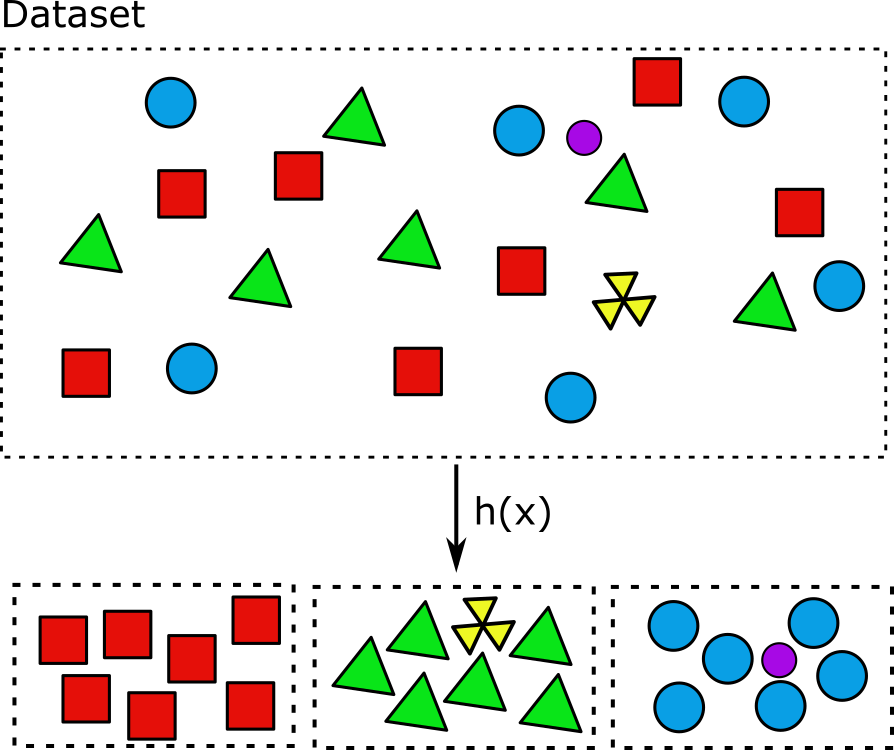
\includegraphics[width=.7\textwidth]{image/new/lsh.png}
\caption{Locality Sensitive Hashing - Documents with similar properties within the dataset are clustered into similar neighbourhood using LSH via the hashing function, h(x). In this example, shapes and colours are used to illustrate documents with similar properties.}
\label{fig:lshexample}
\end{figure}



\subsection{Colour Semantic Extraction }
\label{section:versionOneColorExtract}
%With that in place, this setting effectively performs quantize the range of colours to a fixed number of colour categories while taking advantage of the atom-based structure (Refer to Section \ref{SemanticSegmentation}).

As the background subtraction module has separated the foreground blobs from background scene, these blobs are now assigned a bounding box using the blob's maximum and minimum value on both axis. These bounding box are used to mark the location of the vehicle when a vehicle is detected in the scene. However, due to the background subtraction method adopted, the final foreground blob tend to appear somewhat larger than the actual vehicle footprint.

In order to minimise noise from the bounding box and to obtain a closer estimation of the vehicle's dominant colour, the bounding box is cropped by a factor of 30\% to reduce background noise such as the tar road or vehicles close to it. In order to maintain as much information, the bounding box was not reduced further as that often results in the cropping of the vehicle's windscreen and window regions, thus altering the overall dominant colour.

Upon having the bounding box of the vehicles cropped, the next strategy implemented was to determine the dominant colour of each vehicle by first distinguishing between chromatic and achromatic vehicles. Following similar definition of achromatic colours from Munsell, achromatic colours also known as neutral colours are characterised by the lack of strong hue or chroma values such as black, white and gray colour.

\begin{figure}[htb!]
  \centering
\begin{tabular}{c}
 
\includegraphics[width=0.7\linewidth]{image/retrievalOne/all.png} \\
\end{tabular}
\caption{960 Allocated Colour Bins} \label{fig:hsvAllocated}
\end{figure}

The step to differentiate between chromatic and achromatic vehicles was implemented to overcome the shortcomings of the 960 colour bins proposed for the Colour Term Extraction process. Figure \ref{fig:hsvAllocated} illustrates the colour bins generated, the details on how these colour bins were allocated are discussed later. One of the main drawback of the proposed method was the number of bins used to represent the achromatic colours. From the figure, it is observed that while there are a substantial amount of bins representing the almost-pure-black darker tonnes. However, the number of bins used to represent the lighter shades of achromatic colours are just a fraction of the total bins.
This imbalance, compounded with the noise captured (ie: road, other vehicles, trees) during the dominant colour extraction process made it extremely difficult for vehicles to be match with "White" colour term. Hence, this step was introduced as a measure to counterbalance the weakness of the proposed method.


This process of differentiating chromatic against achromatic vehicles starts off by comparing the cropped image, $I_{crop}$, against a grayscale version of the same image, $I_{gray}$. The conversion from RGB to grayscale is performed using $I_{gray} = 0.299 \cdot I_{crop}[R]+0.587 \cdot I_{crop}[G]+0.114 \cdot I_{crop}[B]$. However, as the grayscale image and RGB image does not have the same number of channels, hence, the grayscale image was converted back to a RGB image prior to the comparison.
The absolute difference between these images were obtained using: $I_{Abs_{diff}} = \mid I_{crop} - I_{gray(RGB)} \mid$. Next, the obtained $I_{Abs_{diff}}$ result was subjected to a threshold process for all three channels in the RGB colour space to produce $I_{threshold}(RGB)$.
The step was done to effectively amplify the difference between the original image and the grayscale image, Pixels, $Pv_{(x,y)}$, with values above the threshold value of 35 were set to the maximum value of 255.
\begin{align*}
\label{eq:threshabsolutediff}
I_{threshold}(x,y)(RGB) = \alpha \cdot (255) \\
\text{where, }
\alpha =
\begin{cases}
1, & Pv_{(x,y)} \geq 35\\
0, & otherwise
\end{cases}
\end{align*}

 Finally, the output of the process was converted back to the grayscale colour space to generate $I_{threshold}(gray)$. The hint of significant values at this stage provides an indication of substantial presence of chromatic hues for this particular vehicle.


\begin{comment}
\begin{align}
\label{eq:achromaticSteps}
I_{ori_{i,j}} = \{R_{i,j},G_{i,j},B_{i,j}\} \\
I_{grayscale}, Y_{i,j} = 0.299 \cdot I_{ori}R_{(x_i,y_j)}+0.587 \cdot I_{ori}G_{(x_i,y_j)}+0.114 \cdot I_{ori}B_{(x_i,y_j)}\\
I_{grayscale(RGB_{i,j})} = \begin{cases}R = Y_{i,j}\\G = Y_{i,j} \\ B = Y_{i,j} \end{cases}\\
Abs_{diff}(R,G,B) = \mid I_{ori} - I_{grayscale(BGR)} \mid \\
Threshold_{Abs_{diff}}, T_{Abs_{diff}} =
\begin{cases}R = \begin{cases}Abs_{diff}R\geq 35, & R =255\\ otherwise, & R =0
\end{cases} \\
G = \begin{cases}Abs_{diff}G\geq 35, & G =255\\ otherwise, & G =0
\end{cases} \\
B = \begin{cases}Abs_{diff}B\geq 35, & B =255\\ otherwise, & B =0
\end{cases}
\end{cases}\\
Threshold_{Abs_{diff(grayscale)}} = \\
0.299 \cdot T_{Abs_{diff}}R_{(x_i,y_j)}+0.587 \cdot T_{Abs_{diff}}G_{(x_i,y_j)}+0.114 \cdot T_{Abs_{diff}}B_{(x_i,y_j)}
\end{align}
\end{comment}

With the interest of differentiating between chromatic and achromatic vehicles, the ratio of non-zero pixel value over the total pixels in an image were obtained. This threshold pivot value, $T_{pivot}$, was empirically set at 18\% where vehicles blobs that exceeds this value were assumed to contain strong chromatic hue. The entire process from the original image to the deduction of whether a vehicle blob was chromatic or achromatic is illustrated using Figure \ref{fig:achromatic_thresh}. This handcrafted algorithm allows the deduction of strong chromatic hues and estimates if a particular vehicle blob belongs to a chromatic or achromatic subset.


\begin{figure}[htb!]
  \centering
\begin{tabular}{c}
 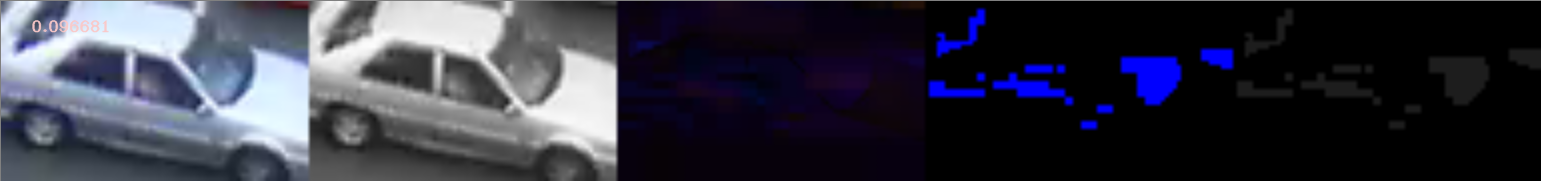
\includegraphics[width=0.9\linewidth]{image/general/achromatic_threshold5.PNG} \\
 (a) Achromatic vehicle (Gray/White) \\
 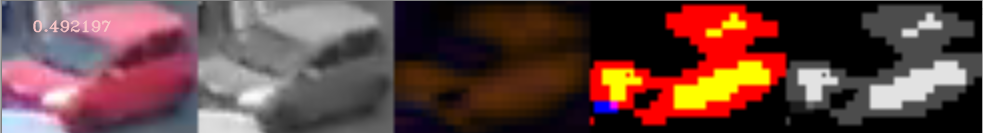
\includegraphics[width=0.9\linewidth]{image/general/achromatic_threshold_color2.PNG}\\
(b) Chromatic vehicle (Red)
\end{tabular}
\caption{(From left) Original image, $I_{crop}$; Grayscale image, $I_{gray}$; Absolute difference, $I_{Abs_{diff}}$; Binary threshold absolute difference, $I_{threshold}(RGB)$; Threshold difference in grayscale, $I_{threshold}(gray)$} \label{fig:achromatic_thresh}
\end{figure}



\paragraph{Achromatic and chromatic colour processing.} Upon determining whether or not the vehicle belongs to the achromatic scale using the $T_{pivot}$ value, the cropped images were then subjected to both the black and white colour filters individually. These simple filters were designed using binary thresholds values empirically set at an intensity levels of 50 and 170 respectively. Next, using a similar fashion, the ratio of non-zero pixels upon filtering were computed. These non-zero percentage ration was used to determine if the vehicle belongs to black, white or gray colour terms. Figure \ref{fig:blackwhite_filter} shows how a white vehicle responds to a black and white filter.


\begin{figure}[htb!]
  \centering
\begin{tabular}{ccc}
 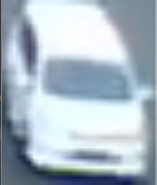
\includegraphics[width=0.22\linewidth]{image/retrievalOne/whitefilter1.png}   &
 
\includegraphics[width=0.22\linewidth]{image/retrievalOne/whitefilter2.png}   &
 
\includegraphics[width=0.22\linewidth]{image/retrievalOne/whitefilter3.png}   \\
(a) Target Vehicle (White) &
(b) Black Filter Response &
(c) White Filter Response \\
\end{tabular}
\caption{Black \& While Filter Response of a White Vehicle} \label{fig:blackwhite_filter}
\end{figure}




 \begin{algorithm}[!ht]
  \caption{Achromatic Colour Term Extraction}
  \label{algo:achromatic}
  \begin{algorithmic}[1]

  \IF{Percentage of White $>$ 25\%  \\
  \hspace{1em} \&\& Percentage of Black $<$ 25\%}
	\STATE Colour Term = White
  \ELSIF {Percentage of Black $>$ 25\%  \\
  \hspace{1em} \&\& Percentage of White $<$ 25\%}
  	\STATE Colour Term = Black
  \ELSE
  	\STATE Colour Term = Gray
  \ENDIF

  \end{algorithmic}
\end{algorithm}


 \begin{algorithm}[!ht]
  \caption{Colour Term Extraction}
  \label{algo:colorExtract}
  \begin{algorithmic}[1]
    \FOR{Each blob in image}
        \STATE Shrink bounding box \& crop image
        \STATE Create a copy of the cropped image in grayscale
        \STATE Compute absolute difference between cropped image \& grayscale image
        \STATE Perform threshold on absolute difference to amplify difference
        \STATE Convert results into grayscale \& calculate no. of non-zero pixels
            \IF{Ratio of non-zero pixels $>$ $T_{pivot}$}
                \STATE // Chromatic Vehicle
                \STATE Calculate 3D HSV histogram
                \STATE Locate maximum bin location of each channel
                \STATE Map the highest bin from each channel to Colour Term
            \ELSE
                \STATE // Achromatic Vehicle
                \STATE Perform black \& white filter
                \STATE Obtain ratio of non-zero pixels from both filters
                \STATE CALL: Achromatic Colour Term Extraction
            \ENDIF

    \ENDFOR
    \STATE Obtain average dominant colour \& return Colour Term
  \end{algorithmic}
\end{algorithm}


As previously mention, this work chose to primarily work on the HSV colour space, especially for the chromatic colour extraction process. First, the cropped image was converted to the HSV colour space. Then, a 3-Dimensional histogram of the cropped image was generated to identify the maximum value of each channel. However, as colours belongs to a spectrum, using a fine-grained histogram is not ideal as the generated output would be spread across a segment. Hence, the HSV channels were quantized into the following settings: 15 Hue bins, 8 Saturation bins and 8 Value bins for the histogram generation.






% Please add the following required packages to your document preamble:
% \usepackage[table,xcdraw]{xcolor}
% If you use beamer only pass "xcolor=table" option, i.e. \documentclass[xcolor=table]{beamer}
\begin{table}[!ht]\centering
\resizebox{\textwidth}{!}{
\begin{tabular}{c|c|c|c|c|c|c|c|c|c|c|c|}
\cline{2-12}
\multicolumn{1}{l|}{}                        & \multicolumn{11}{c|}{\textbf{Similarity(\%) Based on $D_{Euclidean}$ in HSV Colour Space}}                                                                                                                                                                                       \\ \hline
\multicolumn{1}{|c|}{\textbf{Bin/Colour}} & \textbf{Black} & \textbf{Blue} & \textbf{Brown} & \textbf{Gray}                          & \textbf{Green}                         & \textbf{Orange} & \textbf{Pink}                          & \textbf{Purple}                        & \textbf{Red} & \textbf{White} & \textbf{Yellow} \\ \hline
\multicolumn{1}{|c|}{
\begin{tabular}{c}  \\

\includegraphics[width=0.1\linewidth]{image/HSVcolorspace/img_0_4_7.jpg} \\
\textbf{0, 4, 7}
\end{tabular}     }

& 30.46          & 67.06         & 55.74          & 57.51                                  & 70.94                                  & 73.76           & \cellcolor[HTML]{9AFF99}\textbf{92.18} & 71.95                                  & 72.25        & 64.00          & 76.33           \\ \hline

\multicolumn{1}{|c|}{
\begin{tabular}{c}  \\

\includegraphics[width=0.1\linewidth]{image/HSVcolorspace/img_2_4_3.jpg} \\
\textbf{2, 4, 3}
\end{tabular}     }


& 54.07          & 60.33         & 70.03          & 59.16                                  & 66.14                                  & 55.81           & 64.00                                  & \cellcolor[HTML]{9AFF99}\textbf{81.03} & 59.25        & 49.04          & 55.33           \\ \hline

\multicolumn{1}{|c|}{
\begin{tabular}{c}  \\

\includegraphics[width=0.1\linewidth]{image/HSVcolorspace/img_3_7_4.jpg} \\
\textbf{3, 7, 4}
\end{tabular}     }

& 29.70          & 73.77         & 86.97          & 42.04                                  & \cellcolor[HTML]{9AFF99}\textbf{90.03} & 72.85           & 58.01                                  & 78.43                                  & 76.15        & 33.49          & 72.24           \\ \hline
\multicolumn{1}{|c|}{
\begin{tabular}{c}  \\

\includegraphics[width=0.1\linewidth]{image/HSVcolorspace/img_6_2_6.jpg} \\
\textbf{6, 2, 6}
\end{tabular}     }


& 41.35          & 56.33         & 46.77          & \cellcolor[HTML]{9AFF99}\textbf{75.87} & 62.87                                  & 53.88           & 72.91                                  & 62.49                                  & 52.12        & 69.89          & 58.04           \\ \hline



% ----- remove these?

\multicolumn{1}{|c|}{
\begin{tabular}{c}  \\

\includegraphics[width=0.1\linewidth]{image/HSVcolorspace/img_11_0_0.jpg} \\
\textbf{11, 0, 0}
\end{tabular}     } &

\cellcolor[HTML]{9AFF99}\textbf{88.15} &	21.74 &	35.36 &	60.73 &	31.88 &	17.02 &	34.30 &	41.36 &	19.80 &	39.59 &	17.52
\\ \hline

\multicolumn{1}{|c|}{
\begin{tabular}{c}  \\

\includegraphics[width=0.1\linewidth]{image/HSVcolorspace/img_11_0_1.jpg} \\
\textbf{11, 0, 1}
\end{tabular}     }  &
\cellcolor[HTML]{9AFF99}\textbf{83.66} &	26.71 &	37.51 &	67.13 &	36.19 &	22.35 &	41.39 &	45.70 &	24.80 &	47.38 &	23.04
\\ \hline

\multicolumn{1}{|c|}{
\begin{tabular}{c}  \\

\includegraphics[width=0.1\linewidth]{image/HSVcolorspace/img_11_0_2.jpg} \\
\textbf{11, 0, 2}
\end{tabular}     }  &
\cellcolor[HTML]{9AFF99}\textbf{77.20} &	31.13 &	38.69 &	72.71 &	39.75 &	27.21 &	48.22 &	49.15 &	29.27 &	55.12 &	28.11
\\ \hline

\multicolumn{1}{|c|}{
\begin{tabular}{c}  \\

\includegraphics[width=0.1\linewidth]{image/HSVcolorspace/img_11_0_3.jpg} \\
\textbf{11, 0, 3}
\end{tabular}     }  &
70.02 &	34.87 &	38.85 &	\cellcolor[HTML]{9AFF99}\textbf{76.86} &	42.43 &	31.48 &	54.68 &	51.54 &	33.08 &	62.76 &	32.61
\\ \hline

\multicolumn{1}{|c|}{
\begin{tabular}{c}  \\

\includegraphics[width=0.1\linewidth]{image/HSVcolorspace/img_11_0_4.jpg} \\
\textbf{11, 0, 4}
\end{tabular}     }  &
62.53 &	37.82 &	37.98 &	\cellcolor[HTML]{9AFF99}\textbf{78.73} &	44.10 &	35.06 &	60.60 &	52.69 &	36.13 &	70.25 &	36.44
\\ \hline

\multicolumn{1}{|c|}{
\begin{tabular}{c}  \\

\includegraphics[width=0.1\linewidth]{image/HSVcolorspace/img_11_0_5.jpg} \\
\textbf{11, 0, 5}
\end{tabular}     }  &
54.88 &	39.85 &	36.13 &	\cellcolor[HTML]{9AFF99}\textbf{77.73} &	44.67 &	37.83 &	65.69 &	52.53 &	38.30 &	77.42 &	39.47
\\ \hline

\multicolumn{1}{|c|}{
\begin{tabular}{c}  \\

\includegraphics[width=0.1\linewidth]{image/HSVcolorspace/img_11_0_6.jpg} \\
\textbf{11, 0, 6}
\end{tabular}     }  &
47.14 &	40.88 &	33.38 &	74.20 &	44.10 &	39.67 &	69.54 &	51.05 &	39.50 &	\cellcolor[HTML]{9AFF99}\textbf{83.84} &	41.56
\\ \hline

\multicolumn{1}{|c|}{
\begin{tabular}{c}  \\

\includegraphics[width=0.1\linewidth]{image/HSVcolorspace/img_11_0_7.jpg} \\
\textbf{11, 0, 7}
\end{tabular}     }  &
39.35 &	40.84 &	29.83 &	68.98 &	42.43 &	40.49 &	71.62 &	48.38 &	39.665 &	\cellcolor[HTML]{9AFF99}\textbf{88.23} &	42.61
\\ \hline



% ----- remove these?


\end{tabular}}
\caption{Samples of Similarity Score(\%) based on Euclidean Distance in HSV Colour Space, Highlighted in Green is the Highest Scoring Colour Term}
\label{tab:hsvExample}
\end{table}










This setup ends up with a total of 960 bins where each of these bins are assigned a single colour term based on the closest euclidean distance between this bin's colour and the highest scoring ground truth colour term using the HSV colour space. Using this setup, the colour term which corresponds to the bin(h,s,v) which contains the highest number of hits for a given image is assigned. The examples in Table \ref{tab:hsvExample} shows samples of bins and their corresponding similarity score. However, since the vehicles are moving in the outdoor setting, the ambient and directional lighting (from sun and other light sources) contribute to slight variation of colours. To accommodate the varying lighting condition, the dominant colour of each tracked vehicle from each frame was averaged out throughout its trajectory as illustrated in \ref{fig:ADC}.


As the entire process was done repeatedly over every single frame in the video, the colour term of a particular vehicle is saved into the database while it is tracked. As such, a single vehicle could be classified as a variety of colours depending on the location on where the vehicle was tracked. Algorithm \ref{algo:colorExtract} summarises the strategy used for colour semantic extraction process for the \versionOneExt.



\subsection{Motion Semantic Extraction}
\label{subsec:motions9binextract}

In order to extract motion information of vehicles, the initial step of obtaining the foreground objects from the background subtraction method still stands. Upon identifying these foreground objects, the locations of each vehicles are obtained using the centroids using Equation \ref{eq:centroid}. The motions were extracted by naive position displacement inference methods. Next, the centroids of the vehicles from each frame ($P_N$) are stored in a list, \H{L}.

As two subsequent frames is likely to have too little difference, the algorithm was set to wait until the list has at least 10 records of the previous position before extracting the motion information. Algorithm \ref{algo:motion} provides details of this semantic extraction process in pseudo-code. In this work, the motion of a vehicle is quantized into 8 directional bins (in the form of four cardinal directional and four intermediate directional bins) along with another bin which denotes minuscule and negligible motion information. These quantized directions can be categorised into: UP, DOWN, LEFT, RIGHT, LEFT-UP, LEFT-DOWN, RIGHT-UP, RIGHT-DOWN, MOTIONLESS.

Figure \ref{fig:cardinalbins} illustrates this property. Each of this directions are determined using handcrafted parameters which were selected empirically, the displacement values, $X_{displacement}$ \& $Y_{displacement}$ were set to 5 pixels each. If the difference between the current position of the blob and the position 10 frames ago is larger than either $X_{displacement}$ or $Y_{displacement}$, the motion of the vehicle is updated accordingly. The extracted motion semantic is then saved into the database for each frame.

\begin{figure}[H]\centering
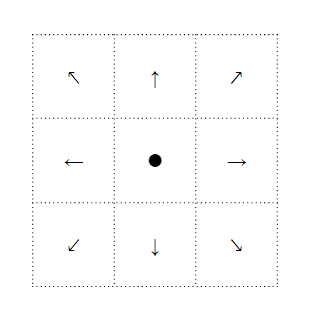
\includegraphics[width=.5\textwidth]{image/new/motion.PNG}
\caption{Directional bins setup}
\label{fig:cardinalbins}
\end{figure}


 \begin{algorithm}[H]
	\caption{Motion Semantic Extraction}
	\label{algo:motion}
	\begin{algorithmic}[1]
		\FOR{Each blob}
		\STATE Save current centroid position ($P_N$) in $List_{motion}$, \H{L}
		\IF{\H{L}.length > 10}
		\STATE Calculate $Difference_x$ and $Difference_y$ using:
		\STATE $Difference_{centroid} = P_N -P_{(N-10)}$
		\IF {Absolute ($Difference_{x}$) > $X_{displacement}$ }
		\IF {$Difference_{x}$ > 0 }
		\STATE Set \textit{Direction(X)} to "LEFT"
		\ELSE
		\STATE Set \textit{Direction(X)} to "RIGHT"
		\ENDIF
		\ENDIF
		\IF {Absolute ($Difference_{y}$) > $Y_{displacement}$ }
		\IF {$Difference_{y}$ > 0 }
		\STATE Set \textit{Direction(Y)} to "UP"
		\ELSE
		\STATE Set \textit{Direction(Y)} to "DOWN"
		\ENDIF
		\ENDIF

		\IF {\textit{Direction(Y)} != NULL AND \textit{Direction(X)} != NULL }
		\STATE Set blob's motion = \textit{Direction(X)} + \textit{Direction(Y)}
		\ELSE
		\IF {\textit{Direction(X)} != NULL }
		\STATE Set blob's motion = \textit{Direction(X) }
		\ELSIF  {\textit{Direction(Y)} != NULL }
		\STATE Set blob's motion = \textit{Direction(Y)}
		\ELSE
		\STATE Set blob's motion = "Motionless"
		\ENDIF
		\ENDIF
		\ENDIF
		\STATE Save blob's current motion into database
		\ENDFOR
	\end{algorithmic}
\end{algorithm}




\section{\versionTwoExt }
\label{section:semantic_chamfer}


\subsection{Overview}

During the course of experimenting with the \versionOneExt, one of the drawbacks identified was that the semantic extraction process was too handcrafted. Although the results could have improved with more tweaking of the parameters and various knobs available, the process of experimenting what works best would be extremely tedious and the end product would not necessarily be extendable to other frameworks depending on the input data.

Along with that, there were several key issues which were identified that could be improved upon. One of the issue pinpointed was that the process of determining whether or not a vehicle belonged to achromatic or chromatic scale was biased. In the dataset on which the experiments were conducted on, there were a lot more achromatic vehicle compared to chromatic vehicle. As the scale was bias, it was easy to manipulate the overall retrieval results by adjusting the parameters to favour the achromatic scale.

The aim of the \versionTwoExt is to provide alternative solutions and improve the performance of the \versionOneExt. In the following subsections, the colour semantic extraction and motion semantic extraction is discussed in detail.



\subsection{Colour Semantic Extraction}
\label{section:versiontwoColor}
As previously discussed in the section \ref{subsec:colorsemantics}, the basic idea of colours is relatively simple for humans, machines on the other hand, have a hard time understanding the concept of colours. In order to extract colour semantics, the initial steps to obtain the Average Dominant colour (ADC) was inherited from the previous method where the bounding box of the detected vehicles from the background subtraction method were cropped.

Next, the dominant colour from each frame was extracted using the maximum bin of the 3-dimension HSV histogram and concatenated. At the end of a vehicle's tracked life cycle, the concatenated dominant colours were averaged out to obtain the ADC. The example in Figure \ref{fig:ADC} illustrates this method while the pseudo-code of the ADC method is described in Algorithm \ref{algo:ADC}.

\begin{figure}[hbt!]\centering
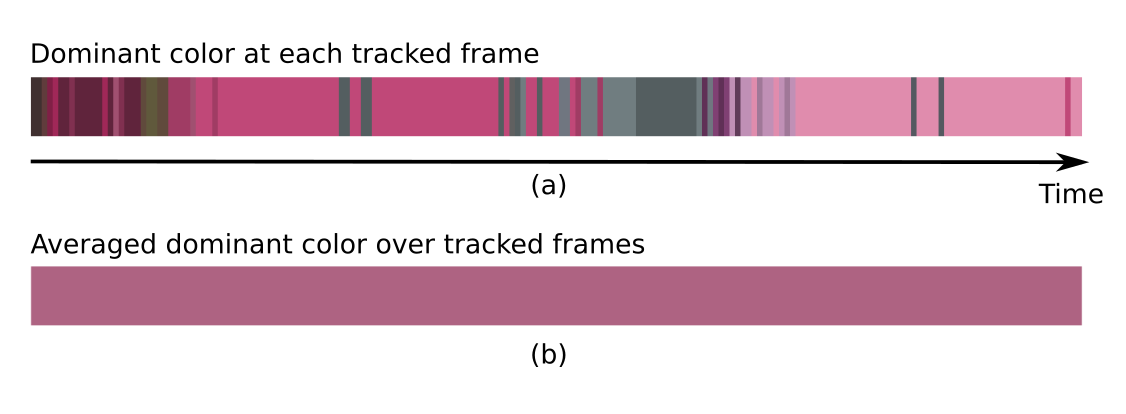
\includegraphics[width=.9\textwidth]{image/general/ADC.png}
\caption{(a) Dominant Colour of the Vehicle at Each Frame; (b) Average Dominant Colour (ADC)}
\label{fig:ADC}
\end{figure}

\begin{algorithm}[H]
  \caption{Average Dominant colour \& Similarity Score Determination}
  \label{algo:ADC}
  \begin{algorithmic}[1]
    \FOR{Each tracked vehicle in the current frame}
        \STATE Shrink bounding box (crop image)
        \STATE Calculate 3D HSV histogram
        \STATE Locate maximum bin location of each channel from histogram
        \STATE Concatenate resulting dominant colours from each frame
        \STATE Obtain the Average Dominant colour (ADC)
        \STATE Measure the difference between ground truth value (Table \ref{table:colorshex}) and ADC
        \STATE Obtain Similarity Score of colour tuple against colour terms
    \ENDFOR
  \end{algorithmic}
\end{algorithm}

In order to reduce the number of parameters and steer clear of handcrafted features such as the one introduced in the previous subsections, instead of assigning one single colour term for each extracted, the similarity score for each colour against all eleven ground truth colours were measured and saved into the database instead. The metrics used to measure the similarity scores between the colours were adopted from the work of Riemersma\cite{riemersma}. This metrics is a low cost estimation of the differences of colours in the LUV linear colour space using RGB values. As the Average Dominant colour was obtained in the HSV colour space, a quick conversion from HSV to RGB colour space was done using Equation \ref{eq:RGBHSVconversion1} to \ref{eq:RGBHSVconversion3}.


%% ---- RGBHSVconversion metric ------------------------------------------------
\begin{equation}
\label{eq:RGBHSVconversion1}
V = \max(R,G,B)
\end{equation}

\begin{equation}
\label{eq:RGBHSVconversion2}
S = \begin{cases}\frac{V - \min(R,G,B)}{V} & , V \neq 0\\
0 & , otherwise \end{cases} \\
\end{equation}

\begin{equation}
\label{eq:RGBHSVconversion3}
H = \begin{cases}
\hspace{2.8em} \frac{60(G-B)}{V-\min(R,G,B)} & ,V = R\\
120 + \frac{60(B-R)}{V-\min(R,G,B)} & ,V = G\\
240 + \frac{60(R-G)}{V-\min(R,G,B)} & ,V = B
\end{cases}
\end{equation}

\centerline{\\$\textit{if } \hspace{.8em}H< 0 \hspace{.8em}\textit{ then } \hspace{.8em}H = H+360.$}





%% ---- RGBHSVconversion metric ------------------------------------------------






According to Riemersma, the benefit of this metrics is that it is a far more stable algorithm where, as quoted, "it does not have a range of colours where it suddenly gives far from optimal results". First, the mean of both the Average Dominant Colour (ADC) and Ground Truth colour (GTC)'s red channel were obtained. Then, this is followed by obtaining the difference, $\Delta$, of all three R, G, and B channels were obtained as well.

In Equation \ref{eq:DiffColorLUV}, the mean of the red channel ($\mean{r}$) is used as a weight for both $\Delta{R}$ and $\Delta{B}$. The details of these equations is described in Equation \ref{eq:RedMeanRGBDiff} and \ref{eq:DiffColorLUV} respectively. Table \ref{tab:luvExample} uses the same example colours as used in Table \ref{tab:hsvExample}, however, the similarity score of the colours were calculated using the metric suggested in Equation \ref{eq:DiffColorLUV} instead of the Euclidean Distance measured in HSV colour space.


%% ---- First metric ------------------------------------------------
\begin{equation}
\begin{split}
\label{eq:RedMeanRGBDiff}
\mean{r} = \frac{C_{1R} + C_{2R}}{2}
\end{split}
% \end{equation}
\quad\quad\quad ; \quad\quad\quad
% \begin{equation}
 \begin{split}
\Delta R = C_{1R} - C_{2R}\\
\Delta G = C_{1G} - C_{2G}\\
\Delta B = C_{1B} - C_{2B}
 \end{split}
\end{equation}

\begin{equation}
\label{eq:DiffColorLUV}
\Delta Colour_{LUV} = \sqrt{(2 + \frac{\mean{r}}{256}) \times \Delta R^{2} + 4 \times \Delta G^{2} + (2 + \frac{255 - \mean{r}}{256}) \times \Delta B^{2} }
\end{equation}




%% ---- First metric ------------------------------------------------



% Please add the following required packages to your document preamble:
% \usepackage[table,xcdraw]{xcolor}
% If you use beamer only pass "xcolor=table" option, i.e. \documentclass[xcolor=table]{beamer}
\begin{table}[!hbt]\centering
\resizebox{\textwidth}{!}{
\begin{tabular}{c|c|c|c|c|c|c|c|c|c|c|c|}
\cline{2-12}
\multicolumn{1}{l|}{}                        & \multicolumn{11}{c|}{\textbf{Similarity(\%) Based on Riemersma's low cost LUV estimation metrics}}                                                                                                                                                                                       \\ \hline
\multicolumn{1}{|c|}{\textbf{Bin/Colour}} & \textbf{Black} & \textbf{Blue} & \textbf{Brown} & \textbf{Gray}                          & \textbf{Green}                         & \textbf{Orange} & \textbf{Pink}                          & \textbf{Purple}                        & \textbf{Red} & \textbf{White} & \textbf{Yellow} \\ \hline
\multicolumn{1}{|c|}{
\begin{tabular}{c}  \\

\includegraphics[width=0.1\linewidth]{image/HSVcolorspace/img_0_4_7.jpg} \\
\textbf{0, 4, 7}
\end{tabular}     }

&
0.00 & 	0.91 & 	28.25 & 	61.27 & 	14.33 & 	67.17 & 	\cellcolor[HTML]{9AFF99}\textbf{70.97} & 	34.74 & 	31.11 & 	25.76 & 	37.78

\\ \hline

\multicolumn{1}{|c|}{
\begin{tabular}{c}  \\

\includegraphics[width=0.1\linewidth]{image/HSVcolorspace/img_2_4_3.jpg} \\
\textbf{2, 4, 3}
\end{tabular}     }


&
34.11 &	22.06 &	\cellcolor[HTML]{9AFF99}\textbf{68.39} &	59.91 &	56.72 &	46.89 &	27.22 &	46.24 &	31.23 &	0.00 &	15.51
\\ \hline

\multicolumn{1}{|c|}{
\begin{tabular}{c}  \\

\includegraphics[width=0.1\linewidth]{image/HSVcolorspace/img_3_7_4.jpg} \\
\textbf{3, 7, 4}
\end{tabular}     }

&
28.13 &	6.53 &	59.41 &	46.70&	\cellcolor[HTML]{9AFF99}\textbf{71.77} &	39.83 &	11.63 &	24.39 &	17.20 &	0.00 &	20.80
\\ \hline
\multicolumn{1}{|c|}{
\begin{tabular}{c}  \\

\includegraphics[width=0.1\linewidth]{image/HSVcolorspace/img_6_2_6.jpg} \\
\textbf{6, 2, 6}
\end{tabular}     }


&
0.00 &	18.72 &	3.55 &	\cellcolor[HTML]{9AFF99}\textbf{70.23} &	27.07 &	16.88 &	44.52 &	18.63 &	0.00 &	46.66 &	27.72
\\ \hline



% ----- remove these?

\multicolumn{1}{|c|}{
\begin{tabular}{c}  \\

\includegraphics[width=0.1\linewidth]{image/HSVcolorspace/img_11_0_0.jpg} \\
\textbf{11, 0, 0}
\end{tabular}     } &

\cellcolor[HTML]{9AFF99}\textbf{89.43}&  	15.88 & 	65.51 & 	10.69 & 	26.97 & 	4.79 & 	0.00& 	35.26 & 	23.58 & 	0.00 & 	0.00
\\ \hline

\multicolumn{1}{|c|}{
\begin{tabular}{c}  \\

\includegraphics[width=0.1\linewidth]{image/HSVcolorspace/img_11_0_1.jpg} \\
\textbf{11, 0, 1}
\end{tabular}     }  &
68.45 &	30.30 &	\cellcolor[HTML]{9AFF99}\textbf{73.87} &	31.62 &	39.47 &	18.66 &	1.26 &	51.17 &	29.17 &	0.00 &	0.00
\\ \hline

\multicolumn{1}{|c|}{
\begin{tabular}{c}  \\

\includegraphics[width=0.1\linewidth]{image/HSVcolorspace/img_11_0_2.jpg} \\
\textbf{11, 0, 2}
\end{tabular}     }  &
47.48 &	39.90 &	\cellcolor[HTML]{9AFF99}\textbf{68.14} &	52.51 &	46.37 &	29.69 &	20.24 &	61.69 &	29.45 &	0.00 &	0.00
\\ \hline

\multicolumn{1}{|c|}{
\begin{tabular}{c}  \\

\includegraphics[width=0.1\linewidth]{image/HSVcolorspace/img_11_0_3.jpg} \\
\textbf{11, 0, 3}
\end{tabular}     }  &
26.52& 	42.30& 	53.27& 	\cellcolor[HTML]{9AFF99}\textbf{73.32}& 	45.52& 	36.31& 	38.11& 	62.02& 	24.32& 	0.14& 	7.44
\\ \hline

\multicolumn{1}{|c|}{
\begin{tabular}{c}  \\

\includegraphics[width=0.1\linewidth]{image/HSVcolorspace/img_11_0_4.jpg} \\
\textbf{11, 0, 4}
\end{tabular}     }  &

5.57 &	36.68 &	35.26 &	\cellcolor[HTML]{9AFF99}\textbf{93.29} &	37.23 &	37.17 &	53.65 &	51.99 &	14.78 &	21.02 &	18.85

\\ \hline

\multicolumn{1}{|c|}{
\begin{tabular}{c}  \\

\includegraphics[width=0.1\linewidth]{image/HSVcolorspace/img_11_0_5.jpg} \\
\textbf{11, 0, 5}
\end{tabular}     }  &

0.00 &	24.52 &	16.04 &	\cellcolor[HTML]{9AFF99}\textbf{83.86} &	23.68 &	32.22 &	64.02 &	36.23 &	2.21 &	42.09 &	26.78

\\ \hline

\multicolumn{1}{|c|}{
\begin{tabular}{c}  \\

\includegraphics[width=0.1\linewidth]{image/HSVcolorspace/img_11_0_6.jpg} \\
\textbf{11, 0, 6}
\end{tabular}     }  &

0.00 &	8.81 &	0.00 &	63.23 &	7.49 &	22.24 &	\cellcolor[HTML]{9AFF99}\textbf{63.64} &	18.07 &	0.00 &	62.88 &	29.66

\\ \hline

\multicolumn{1}{|c|}{
\begin{tabular}{c}  \\

\includegraphics[width=0.1\linewidth]{image/HSVcolorspace/img_11_0_7.jpg} \\
\textbf{11, 0, 7}
\end{tabular}     }  &

0.00 &	0.00 &	0.00 &	42.41 &	0.00 &	8.99 &	53.11 &	0.00 &	0.00 &	\cellcolor[HTML]{9AFF99}\textbf{83.42} &	27.06
\\ \hline



% ----- remove these?


\end{tabular}}
\caption{Samples of Similarity Score(\%) based on Riemersma's low cost LUV estimation metrics, Highlighted in Green is the Highest Scoring colour Term}
\label{tab:luvExample}
\end{table}

The usage of all eleven colour terms to describe an ADC is essential as some colours bears high similarity against the other. A good example would be between pink and red colour; while they are essentially two different colours, however, both these colours belong to a relatively similar hue family. Hence, the similarity score between both these red and pink colour would rather high. This setup allows colours which are visually similar to be ranked higher when the video shots are retrieved using the retrieval engine.

Based on the similarity score (\%) obtained using Riemersma's low cost LUV estimation metrics recorded in Table \ref{tab:luvExample}, the initial analysis of the data shows that distinction between contrasting colour terms are rather clear especially when comparing against the data in Table \ref{tab:hsvExample}.




\begin{figure}[hbt!]\centering
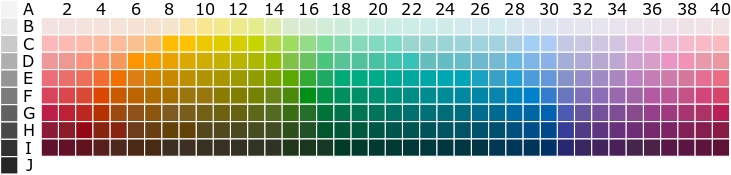
\includegraphics[width=.9\textwidth]{image/analysis/munsell_o.png}
\caption{Munsell 330 Colour Chip}
\label{fig:munsell_ori330}
\end{figure}


\begin{comment}
\begin{figure}[htb!]
  \centering
\begin{tabular}{cc}
 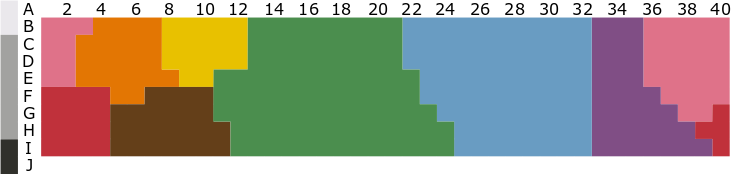
\includegraphics[width=0.45\linewidth]{image/analysis/munsell_a.png}   &
 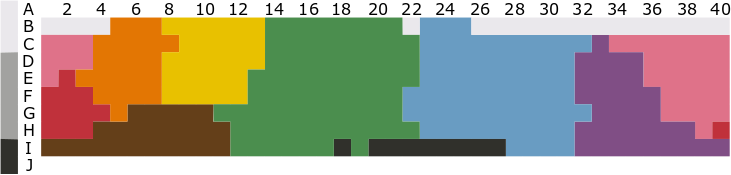
\includegraphics[width=0.45\linewidth]{image/analysis/munsell_b.png}   \\
(a) Parametric model &
(b) PLSA-individual  \\
 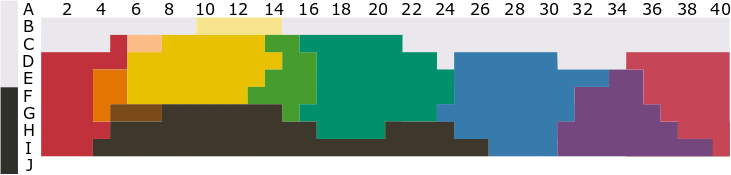
\includegraphics[width=0.45\linewidth]{image/analysis/munsell_e.png}  &
 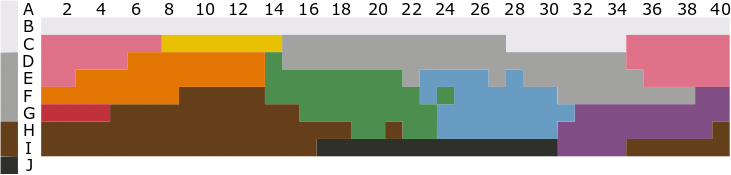
\includegraphics[width=0.45\linewidth]{image/analysis/munsell_d.png}   \\
(c) Linguistic Approach &
(d) Our method \\
\end{tabular}
\caption[Comparison of the Munsell 330 Colour Chips and the Assigned Colour Terms]{Comparison of the Munsell 330 Colour Chips and the Assigned Colour Terms. (a) Parametric model. Image reproduced from \citeA{benavente2008parametric}; (b) PLSA-individual. Image reproduced from \citeA{van2009learning}; (c) Linguistic Approach. Image reproduced from \citeA{zaslavsky2018efficient}; (d) Proposed Method } \label{fig:munsell_compare}
\end{figure}
\end{comment}



\begin{figure}[htb!]
  \centering
\begin{tabular}{c}
 (a) Parametric model \\
 \includegraphics[width=0.7\linewidth]{image/analysis/munsell_a.png}   \\
 (b) PLSA-individual  \\
 \includegraphics[width=0.7\linewidth]{image/analysis/munsell_b.png}   \\
 (c) Linguistic Approach, Before Compression \\
 \includegraphics[width=0.7\linewidth]{image/analysis/munsell_c.png}   \\
 (d) Linguistic Approach, After Compression \\
 \includegraphics[width=0.7\linewidth]{image/analysis/munsell_e.png}  \\
 (e) Proposed method\\
 \includegraphics[width=0.7\linewidth]{image/analysis/munsell_d.png}   \\
\end{tabular}
\caption[Comparison of the Munsell 330 Colour Chips and the Assigned Colour Terms]{Comparison of the Munsell 330 Colour Chips and the Assigned Colour Terms. (a) Parametric model. Image reproduced from \citeA{benavente2008parametric}; (b) PLSA-individual. Image reproduced from \citeA{van2009learning}; (c, d) Linguistic Approach (Before \& After compression). Image reproduced from \citeA{zaslavsky2018efficient}; (e) Proposed Method } \label{fig:munsell_compare}
\end{figure}


Figure \ref{fig:munsell_ori330} shows the original Munsell 330 Colour chips which contains 10 achromatic colour chips and 320 chromatic colour chips.
The 320 chromatic chips are 40 hues (at full saturation) which are evenly spaced out with 8 different levels of lightness (value) for each hue-value pair (\cite{kay2009world}).
These chips are also known as the World Colour Survey (WCS) stimulus palette.
Figure \ref{fig:munsell_compare} shows the comparison of how the WCS stimulus palette were assigned colour terms using different methods; (a)Parametric model by \citeA{benavente2008parametric}; (b) Probabilistic Latent Semantic Analysis (PLSA) - individual by \citeA{van2009learning}; (c, d) Linguistic and Data Compression approach by \citeA{zaslavsky2018efficient}; (e) Proposed method - which assigns the colour term that contains achieved the highest similarity score (\%) using Riemersma's low cost LUV estimation metrics.

When comparing the parametric model (a) and PLSA model (b) against the linguistic approach (c) and proposed method (e), it is noted that the achromatic tones were given more room to express its nature of low saturation value. However, as the assigning of colour terms are subjective to individuals, is it difficult to measure how well each method performed against each other. Hence, a user study of 77 individuals was conducted to determine which method performed the best to classifying colours from the WCS stimulus into colour terms (Figure \ref{fig:munsell_compare}). The results from the user study is tabulated in Table \ref{tab:munsell_result}.

\begin{table}[H]\centering
\begin{tabular}{|l|c|c|}
\hline
\textbf{Method}                             & \textbf{\# of votes} & \textbf{Percentage (\%)} \\ \hline
(a) Parametric model                        & 17                   & 22.08              \\ \hline
(b) PLSA-individual                         & 20                   & 25.97              \\ \hline
(c) Linguistic Approach, Before Compression & 4                    & 5.19              \\ \hline
(d) Linguistic Approach, After Compression  & 24                   & 31.17              \\ \hline
(e) Proposed method                         & 12                   & 15.58              \\ \hline
\end{tabular}
\caption{User study: Understanding Users' Preference on How Colour Terms Should Be Allocated}
\label{tab:munsell_result}
\end{table}

\vspace{-2em}

While the results tabulated does not favour the proposed method, the overall results shows and agrees with the hypothesis that the division of colour terms according to the colour chips are widely subjective. However, the linguistic approach after compression (d) received the highest number of votes.
However, this approach of testing does not reflect the total capability of the proposed method as the proposed method returns a set of probability for each of the colour terms instead of one final value.



\subsection{Motion Semantic Extraction}
\label{subsec:chamferdistancemotionextraction}

With the intention of extracting motion information from the input video data, the spatio-temporal cuboids or \emph{atoms} were adopted here. Contrary to the framework used in \versionOneExt's motion extraction framework, instead of grouping the motions into 9 directional bins, only the location information of the vehicle is saved. This eliminates the use of handcrafted parameters while maintaining important low level semantics which can be used to represent motion information.


\begin{equation}
\label{eq:centroid}
(Centroid_x, Centroid_y) = (\frac{BB_{x}+BB_{width}}{2} , \frac{BB_{y}+BB_{height}}{2})
\end{equation}
\vspace{-2em}
\begin{align*}
    \text{where BB is the Bounding Box of the vehicle}
\end{align*}

As the background subtraction method has identified the vehicle's location, the centroid of the vehicle can be easily computed by inferring the data from bounding box using Equation \ref{eq:centroid}. Using the \emph{atoms} structure as introduced in Section \ref{section:framework}, each \emph{atom} can be uniquely identified using its' respective identifier via its x, y, and t-coordinate. A vehicle's trajectory, $P$, can be denoted using the collection of  vehicle's centroid from each tracked frame in its life cycle. In this framework, the exact motion of the vehicle held lesser importance when compared to the locality of the vehicle itself.

\begin{align}
    P &= \{ (x_i, y_i, t_i), (x_{i+1}, y_{i+1}, t_{i+1}), (x_{i+2}, y_{i+2}, t_{i+2}), \dotsb,(x_{i+n}, y_{i+n}, t_{i+n})\}  \nonumber \\
      &= \{ t_{p1}, t_{p2}, t_{p3}, \dotsb, t_{pn}\}
\end{align}


Now, in order to determine the motion of the vehicle, the order and sequence of the centroids' t-coordinates was used to represents the motion and the trajectory, $P$, of a vehicle. Figure \ref{fig:motionExample} illustrates the property of this setup which allows trajectories of vehicles to be identified by only using the centroid information. Upon obtaining the location of the centroids, the x \& y-coordinate can be inferred as the atom's width and heights were predefined. Finally, the sequence of the t-coordinate along with the x \& y-coordinates are written into the database as a means of collecting motion information.

\begin{figure}[hbt!]\centering
\includegraphics[width=.9\textwidth]{image/general/trajectorysample2.png}
\caption{Collection of a Vehicle's Centroid to Represent the Vehicle's Motion}
\label{fig:motionExample}
\end{figure}

As a vehicle in the car park scene generally does not move in an irregular motion, the sequence information of the vehicle's centroid holds sufficient clue for the reconstruction and estimation of a vehicle's trajectory within the car park scene. This setup also allows reduction of overhead computational cost and storage space which might occur when converting these centroid information into finer vector features.

\section{Summary}
In this chapter, two different semantic extraction methods were proposed. The semantics that were extracted includes the time date information, colour, motion, object type as well as the size of the objects. Both methods employed a slightly different method of extracting the colour and motion information, the performance of these methods will be discussed in Section \ref{section:retrievalengine}.

For the extraction of vehicle colour semantics, in comparison with the existing methods described in Section \ref{section:litreview}, this work proposed a method that works on videos with relatively low resolution. Next, analysis were done on several colour term mapping methods against the WCS stimulus palette. Given that the mapping of these colour terms is subjective to individual's liking, a user study was perform. The results shows most users prefers the colour model proposed by \citeA{zaslavsky2018efficient} after compression.
In the future, the colour term mapping function can be potentially improved so that the results would resemble the best colour mapping function.

